\newpage
\section{Dijkstra's Algorithm - Shortest Path}
\noindent
In this section we will discuss finding the shortest path among a weighted system of relationship.

\begin{theo}[Dijkstra's Algorithm]
    
    \textbf{Proposition:} Suppose that there is a shortest path from nodes $u\to v$. Then any
    sub-path between these nodes, say $x\to y$, is also the shortest path.\\

    \noindent
    \textbf{Algorithm:} Given a weighted graph $G$ and a source node $s$, 
    \begin{enumerate}
        \item [(i.)] Keep track of all the distances between any node $u$ and $s$.
        \item [(ii.)] Start with $s$ and find the next shortest path $u$
        \item [(iii.)] Update the distance between $s$ and $u$ if it is the shortest path.
        \item [(iv.)] Recursively preform steps (ii) and (iii) setting $u$ as the new $s$, updating the original $s$ by the sum of the branch.
    \end{enumerate}

    \noindent
    Moreover on (iii.), as we re-visit $s$: If we find a new shortest path on a different branch, any previous solution is overwritten.
\end{theo}

\vspace{-.5em}
\begin{Tip}
    The `ij' in Dijkstra's pronounced as the `i' in ``kite''.
\end{Tip}

\begin{Proof}[Proof of Correctness for Dijkstra's Algorithm]

    \textbf{Invariant:} For each node $u \in S$, $d(u)$ is the length of a shortest $s \leadsto u$ path.\\
    \textbf{Proof} [by induction on $|S|$]:
    
    \textbf{Base case:} $|S| = 1$ is true since $S = \{s\}$ and $d(s) = 0$.
    
    \textbf{Inductive hypothesis:} Assume true for $|S| = k \geq 1$.
    \begin{itemize}
        \item Let $v$ be the next node added to $S$, and let $(u, v)$ be the final edge.
        \item A shortest $s \leadsto u$ path plus $(u, v)$ is an $s \leadsto v$ path of length $\pi(v)$.
        \item Consider any $s \leadsto v$ path $P$. We show that it is no shorter than $\pi(v)$.
        \item Let $(x, y)$ be the first edge in $P$ that leaves $S$, and let $P'$ be the subpath to $x$.
        \item $P$ is already too long as soon as it reaches $y$.
    \end{itemize}
    \[
    \ell(P) \geq \ell(P') + \ell(x, y) \geq d(x) + \ell(x, y) \geq \pi(y) \geq \pi(v)
    \]
    \noindent
    Thus, the algorithm is correct.
    \end{Proof}
    
\newpage

\noindent
To visualize our proof consider paths the following diagram:
\begin{figure}[h]
    \begin{center}
      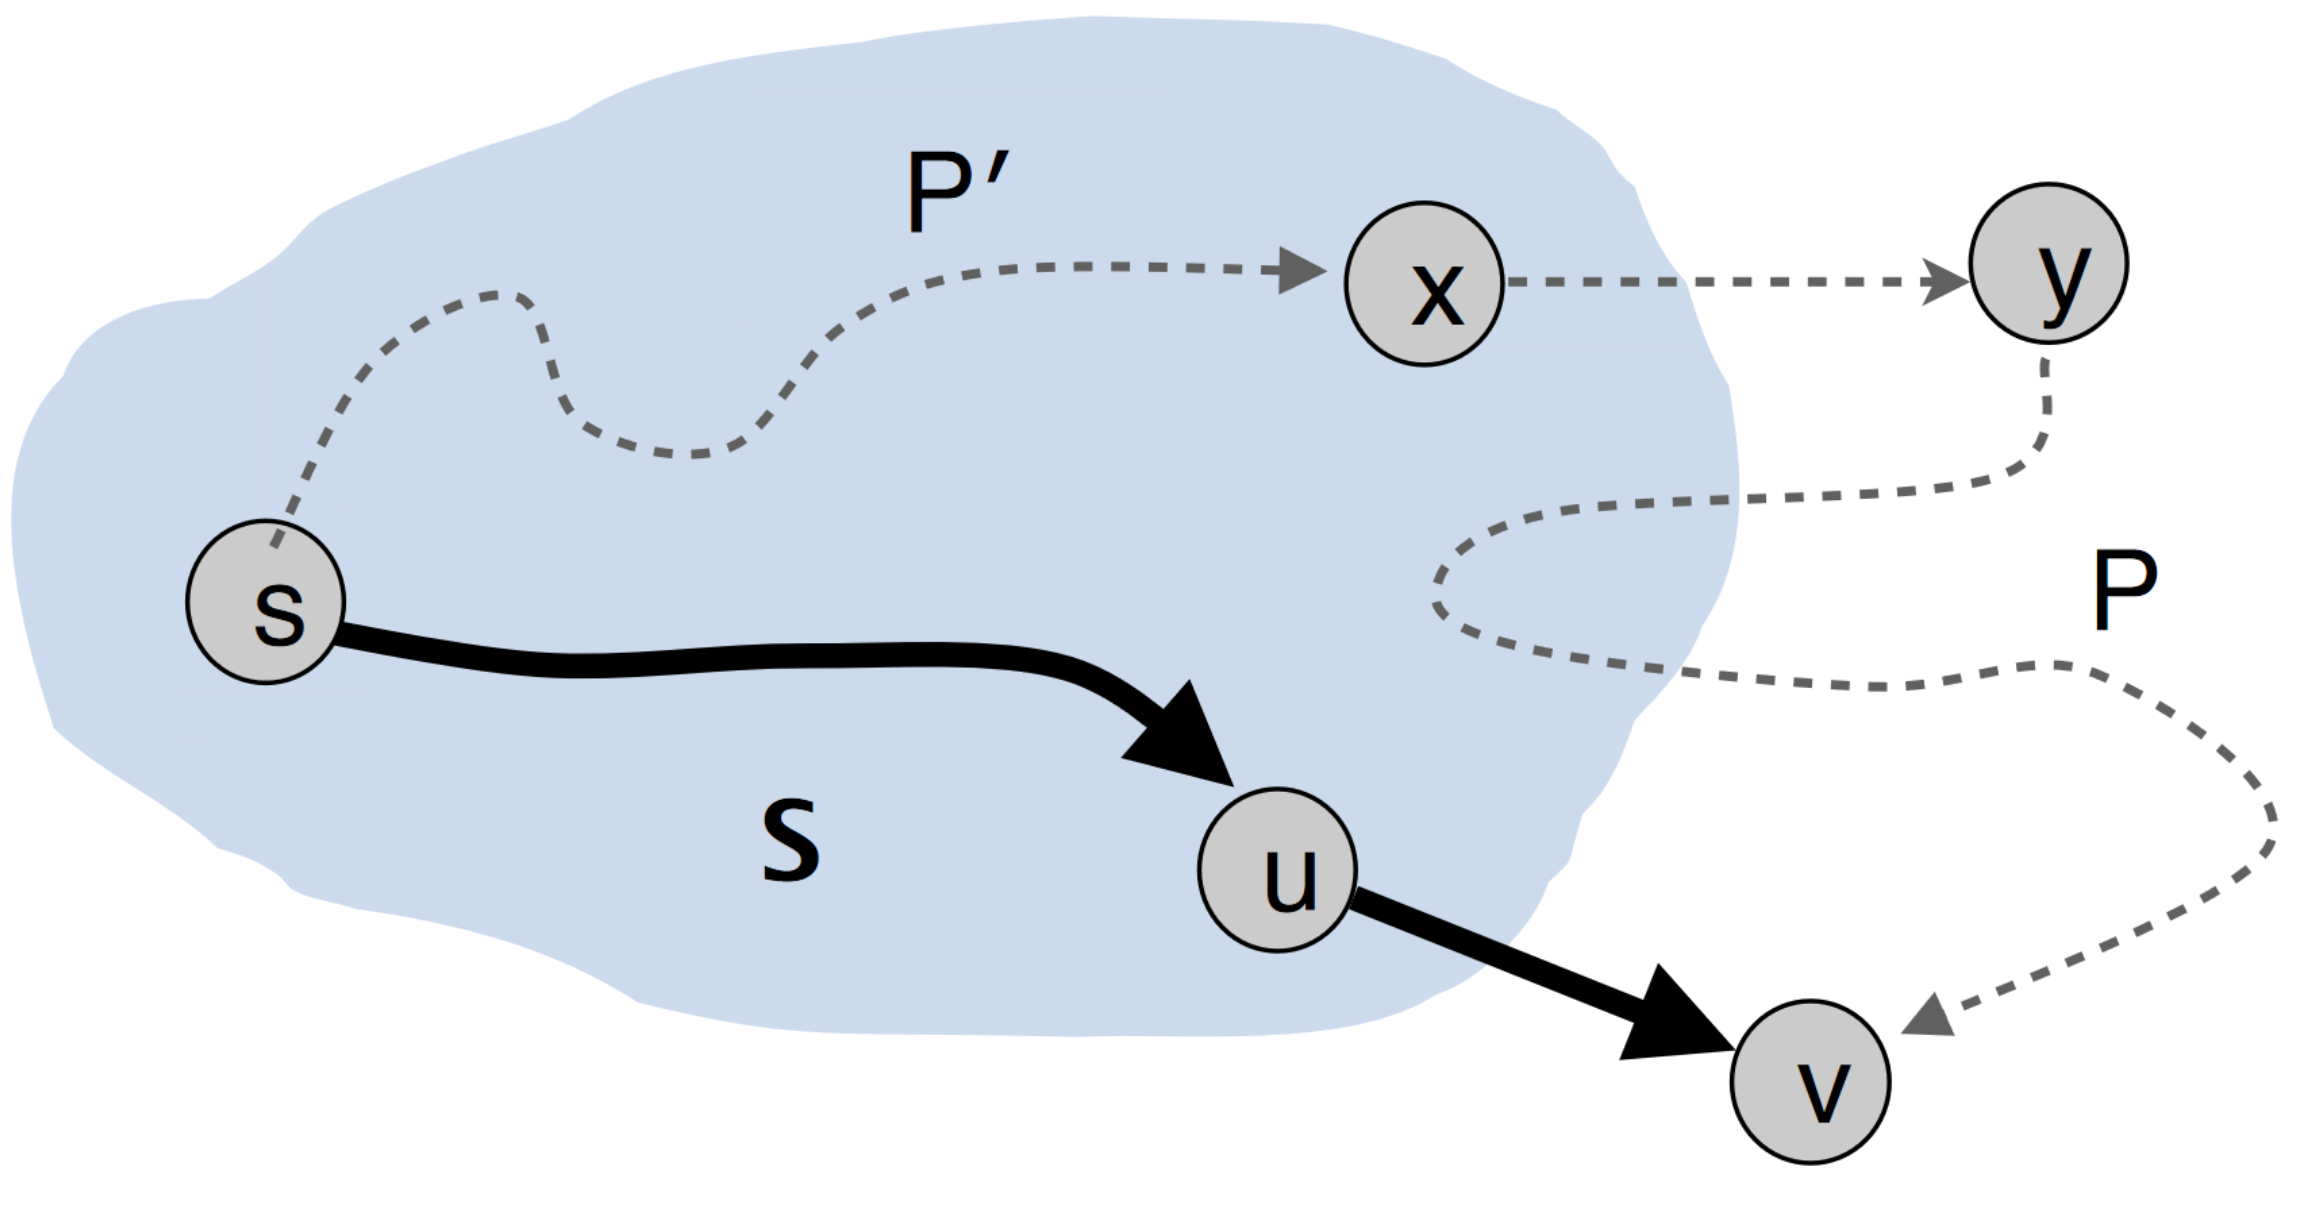
\includegraphics[height=1.5in]{./Sections/sched/dstra/dstra_proof.png}
    \end{center}
     \caption{A system of subset paths (blue), and an exact point of exit $u\to v$ and $x\to y$}\label{fig:dstra_proof}
\end{figure}

\noindent
Since $u\to y$ and $x\to y$ are at the same exact point of exit, i.e., say $s\to v\cong s\to y$, then to go from $y\to v$ must take some additional step.
Therefore, $s\to y\to v$ is longer.\\
\textbf{Example:} Let $s\to y:= 3$ and $s\to v:= 3$, and all steps take $1$.
Then $s\to y\to v = 4$, while $s\to v = 3$. Therefore $s\to v$ is the shortest path.

\noindent
We take the Figure

\begin{figure}[h!]
    \centering
    
    % First subfigure
    \begin{subfigure}{0.35\textwidth}
        \centering
        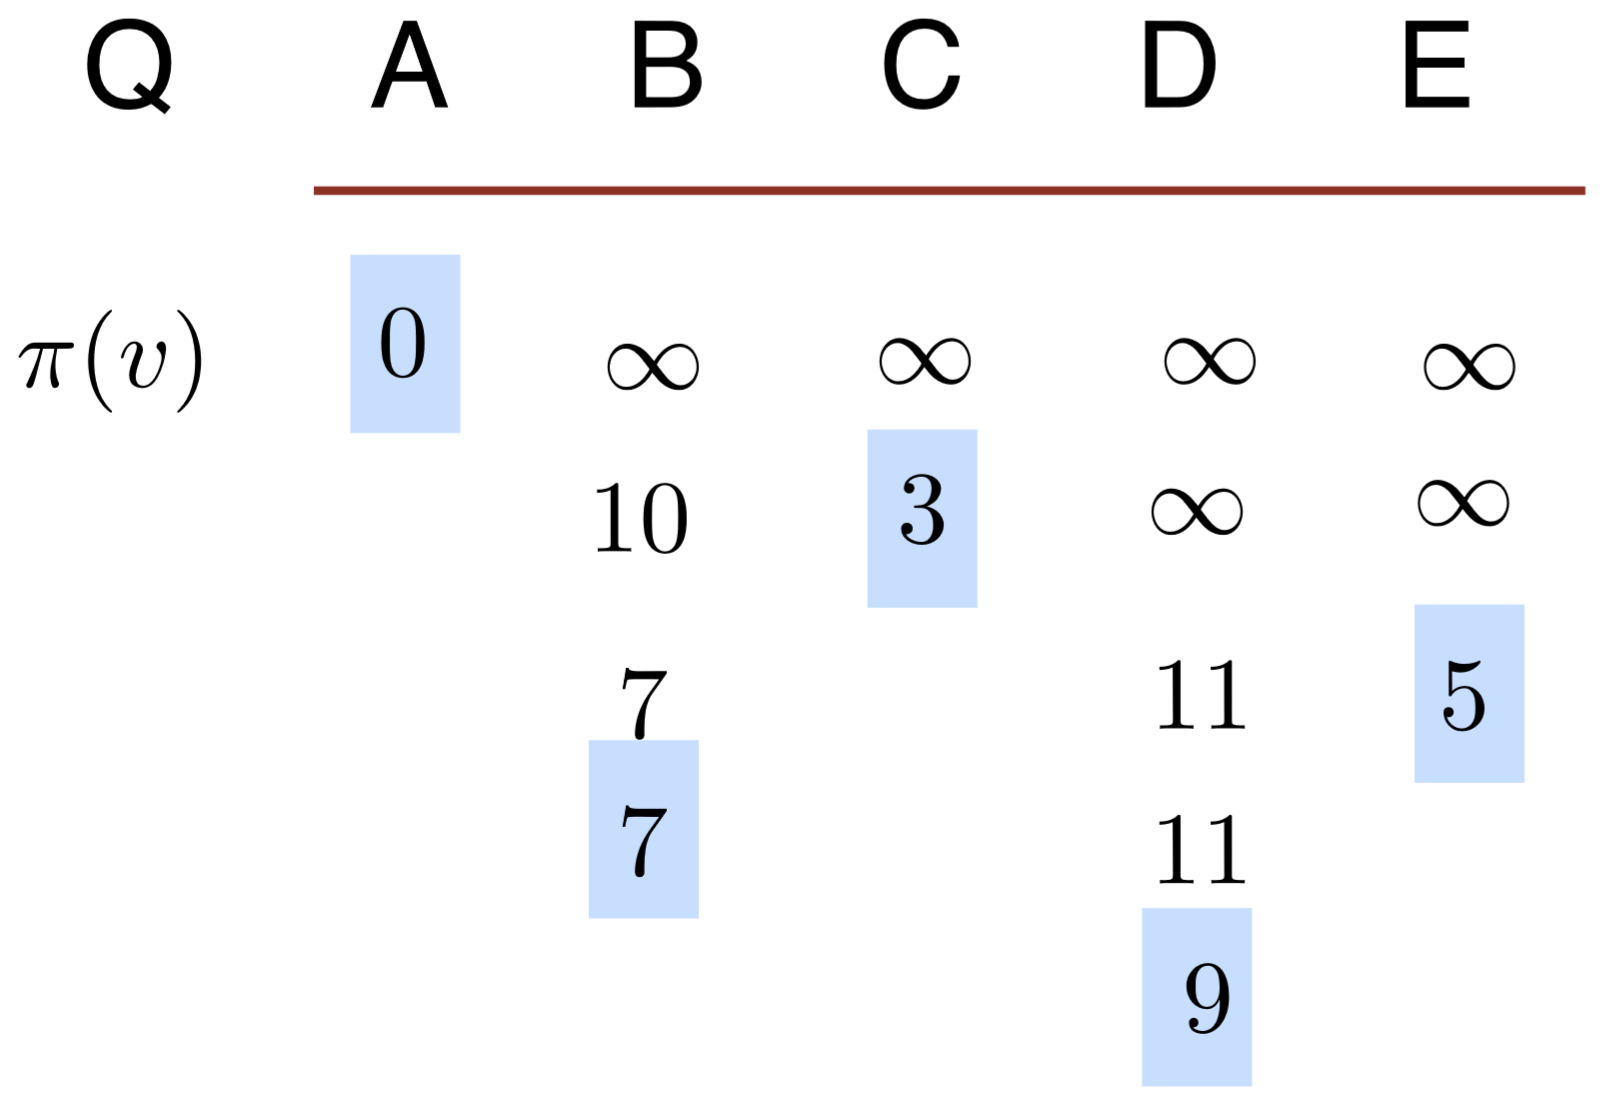
\includegraphics[width=\linewidth]{./Sections/sched/dstra/w_dist.png}
        \caption{Distances from $s$ to each node, shortest paths in blue.}
        \label{fig:subfig1}
    \end{subfigure}
    \quad % Adds space between the two subfigures
    
    % Second subfigure
    \begin{subfigure}{0.45\textwidth}
        \centering
        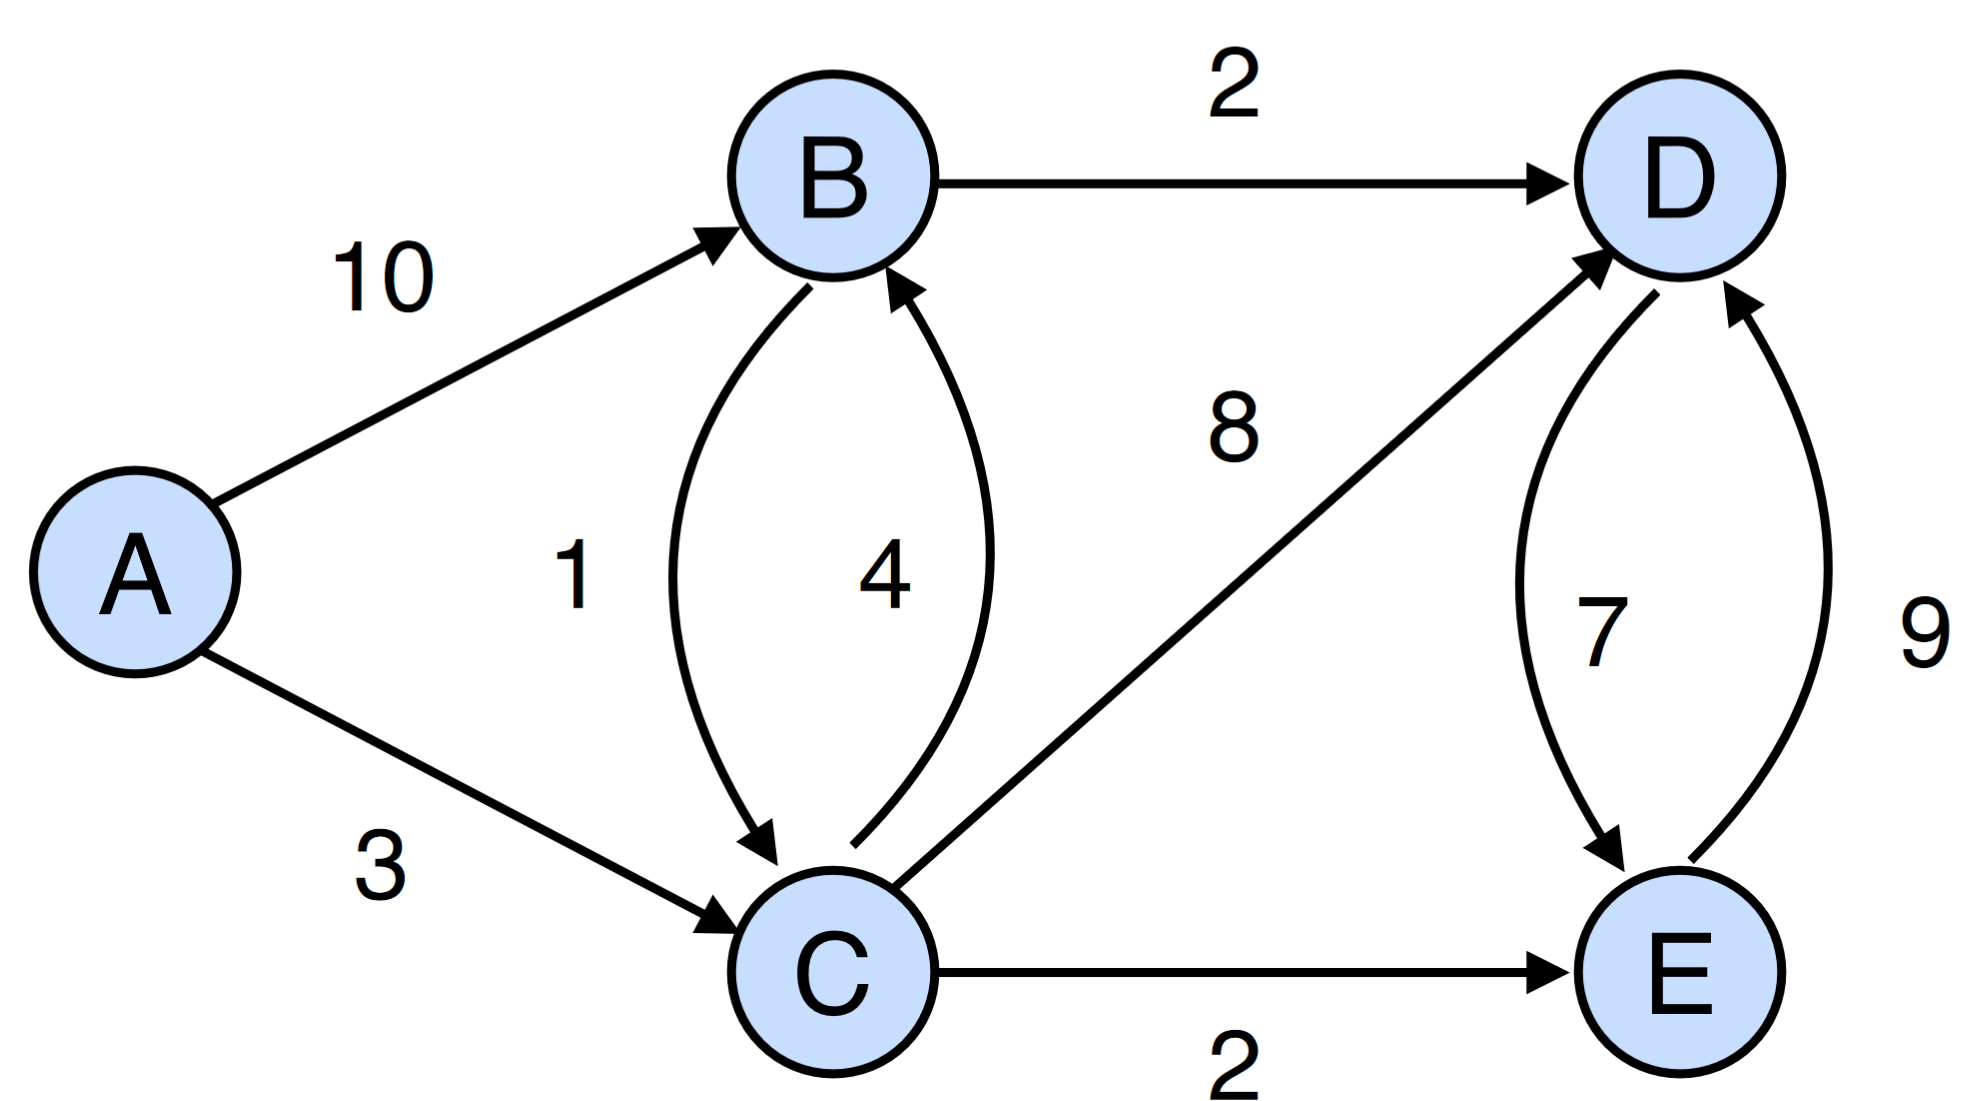
\includegraphics[width=\linewidth]{./Sections/sched/dstra/w_graph.png}
        \caption{A weighted graph relating to Figure (a)}
        \label{fig:subfig2}
    \end{subfigure}
    
    \caption{A weighted graph and its shortest paths.}
    \label{fig:combined_figure}
\end{figure}
\noindent
In figure (\ref{fig:subfig1}), the first row is $0$ as $s\to s$, other nodes are assumed $\infty$,i.e., undefined. Each subsequent row finds the next shortest path, while 
updating the table about information it gathers.


\newpage
\begin{Func}[Dijkstra Algorithm - \texttt{Dijkstra($G, s$)}]

    Finds the shortest path in a weighted directed graph.

    \vspace{.5em}
    \noindent
    \textbf{Input:} A graph $G = (V, E)$ with adjacency list $G[u][v] = l(u, v)$ and source node $s$.\\
    \textbf{Output:} Shortest distances $d[u]$ and parent nodes for paths.

    \begin{algorithm}[H]
        \SetAlgoLined
        \SetKwProg{Fn}{Function}{:}{\KwRet{$d, parents$}}
        \Fn{\texttt{Dijkstra($G, s$)}}{
            $\pi \gets \{\}$\tcp*{hash table, current best list for $v$}
            $d \gets \{\}$\tcp*{hash table, distance of $v$}
            $parents \gets \{\}$\tcp*{parents in shortest path tree}
            $Q \gets \text{PQ()}$\tcp*{priority queue to track minimum $\pi$}

            $\pi[s] \gets 0$\;
            $Q.\texttt{INSERT}(\langle 0, s \rangle)$\;

            \For{$v \neq s$ in $G$}{
                $\pi[v] \gets \infty$\;
                $Q.\texttt{INSERT}(\langle \pi[v], v \rangle)$\;
            }

            \While{$Q$ is not empty}{
                $\langle \pi[u], u \rangle \gets \texttt{EXTRACT-MIN}(Q)$\;
                $d[u] \gets \pi[u]$\;
                \For{$v \in G[u]$}{
                    \If{$\pi[v] > d[u] + l(u, v)$}{
                        $\texttt{DECREASE-KEY}(\langle \pi[v], v \rangle, \langle d[u] + l(u, v), v \rangle)$\;
                        $\pi[v] \gets d[u] + l(u, v)$\;
                        $parents[v] \gets u$\;
                    }
                }
            }
        }
    \end{algorithm}

    \noindent
    \textbf{Time Complexity:} $O(m\log n)$ where $m$ is the number of edges and $n$ is the number of nodes, assuming $G$ is connected $(n-1\leq m)$; Otherwise,
    $O((n+m)\log n)$.\\
    \textbf{Space Complexity:} $O(n+m)$ storing the hash-table of the graph and priority queue.
\end{Func}

\noindent
However we have one problem with Dijkstra's algorithm, it does not work with negative weights.
\begin{theo}[Dijkstra's Algorithm and Negative Weights]
    
    Dijkstra's algorithm does not work with negative weights. This is because it assumes that the shortest path is the sum of the shortest paths. Therefore,
    if the algorithm believes it has found the shortest path, it assumes any further traversals will only increase the path length.
\end{theo}

\newpage

To illustrate the deterioration of Dijkstra's algorithm:

\begin{figure}[h]
    \begin{center}
      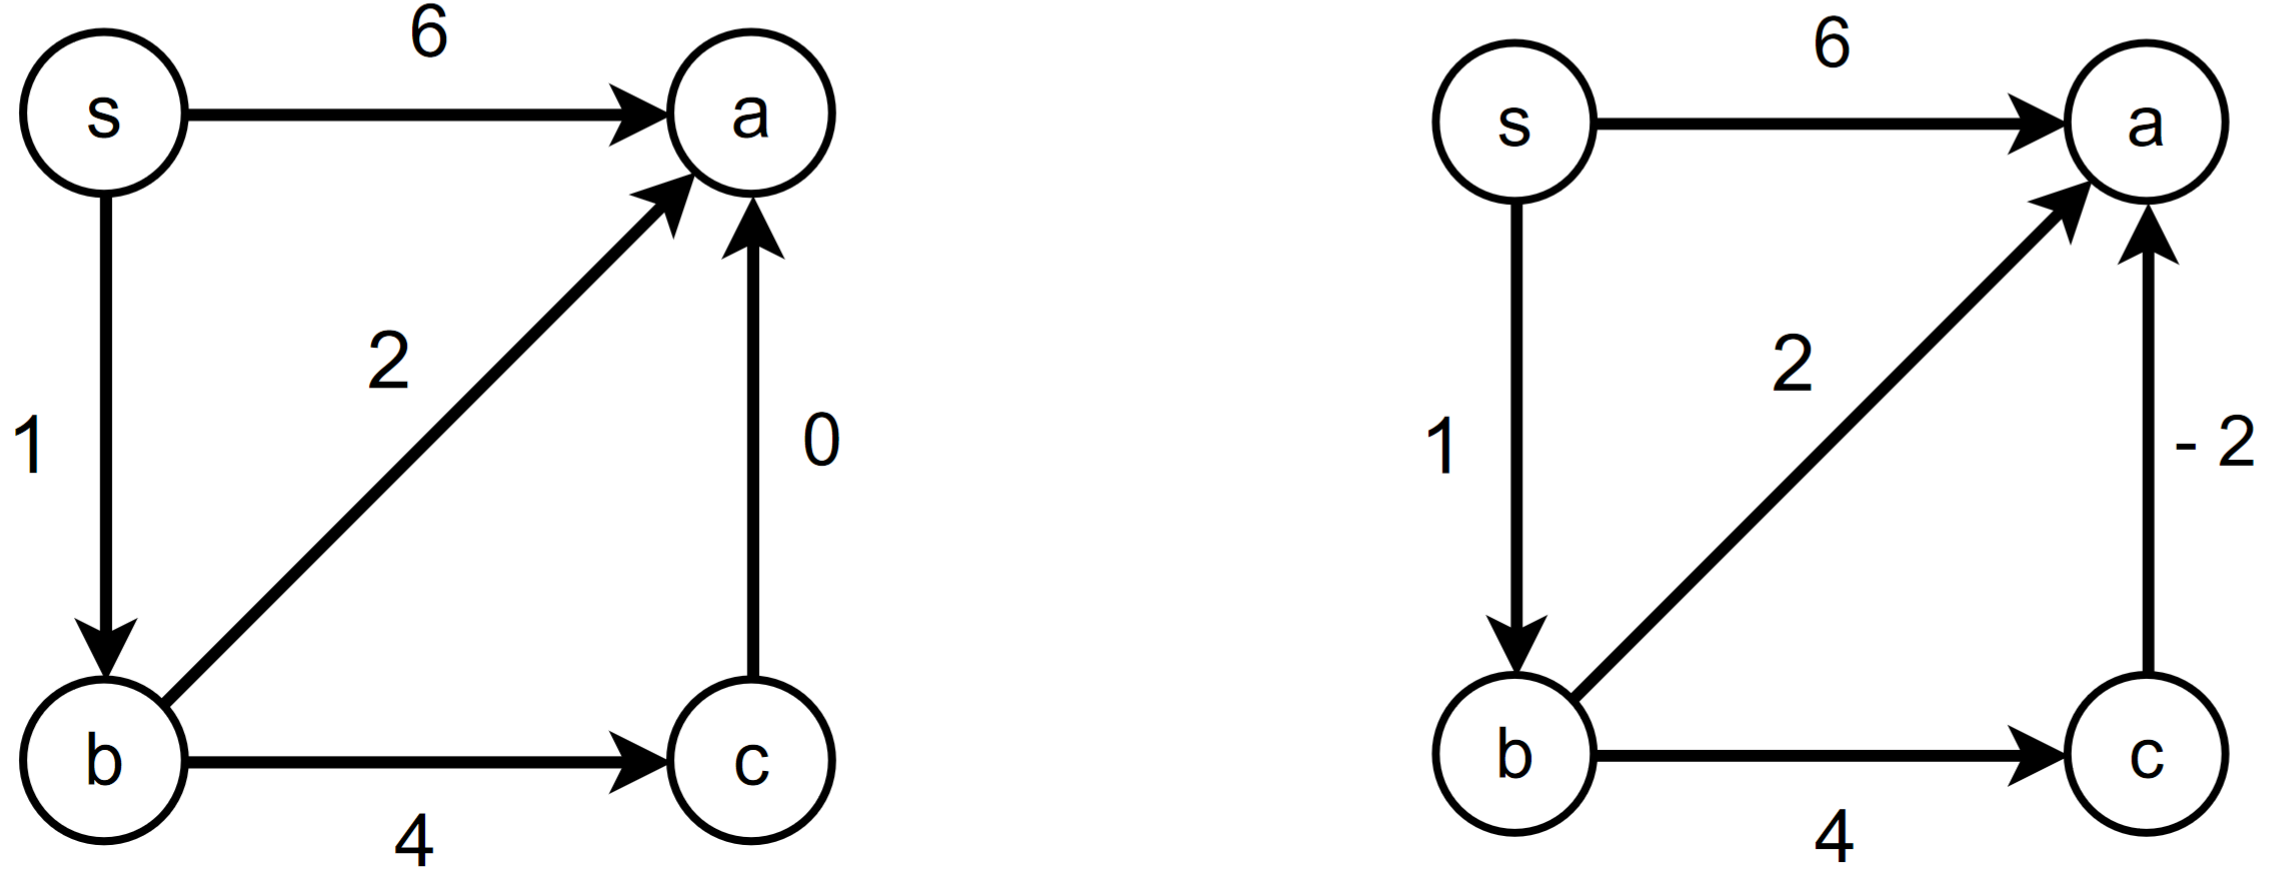
\includegraphics[height=1.5in]{./Sections/sched/dstra/dstra_neg.png}
    \end{center}
     \caption{Shows two weighted graphs, one positive, and the other negative.}\label{fig:dstra_neg}
\end{figure}

\noindent
In Figure (\ref{fig:dstra_neg}), our negative graph will never figure out the shortest path ($s\to b\to c\to a$=1). It 
will always assume $(s\to b\to a=3)$ is the shortest path. As when it looks at $c=4$, it will think that it's 
impossible to yield any shorter of a path $3$ as anything beyond $4$ must be larger.